\pdfbookmark{Общая характеристика работы}{characteristic}             % Закладка pdf
\section*{Общая характеристика работы}

\newcommand{\actuality}{\pdfbookmark[1]{Актуальность}{actuality}\underline{\textbf{\actualityTXT}}}
\newcommand{\progress}{\pdfbookmark[1]{Разработанность темы}{progress}\underline{\textbf{\progressTXT}}}
\newcommand{\aim}{\pdfbookmark[1]{Цели}{aim}\underline{{\textbf\aimTXT}}}
\newcommand{\tasks}{\pdfbookmark[1]{Задачи}{tasks}\underline{\textbf{\tasksTXT}}}
\newcommand{\aimtasks}{\pdfbookmark[1]{Цели и задачи}{aimtasks}\aimtasksTXT}
\newcommand{\novelty}{\pdfbookmark[1]{Научная новизна}{novelty}\underline{\textbf{\noveltyTXT}}}
\newcommand{\influence}{\pdfbookmark[1]{Практическая значимость}{influence}\underline{\textbf{\influenceTXT}}}
\newcommand{\methods}{\pdfbookmark[1]{Методология и методы исследования}{methods}\underline{\textbf{\methodsTXT}}}
\newcommand{\defpositions}{\pdfbookmark[1]{Положения, выносимые на защиту}{defpositions}\underline{\textbf{\defpositionsTXT}}}
\newcommand{\reliability}{\pdfbookmark[1]{Достоверность}{reliability}\underline{\textbf{\reliabilityTXT}}}
\newcommand{\probation}{\pdfbookmark[1]{Апробация}{probation}\underline{\textbf{\probationTXT}}}
\newcommand{\contribution}{\pdfbookmark[1]{Личный вклад}{contribution}\underline{\textbf{\contributionTXT}}}
\newcommand{\publications}{\pdfbookmark[1]{Публикации}{publications}\underline{\textbf{\publicationsTXT}}}


{\actuality} Теория идеальной пластичности является одним из фундаментальных разделов механики твердого деформируемого тела.
Главной особенностью соотношений теории пластичности является нелинейность исходных дифференциальных уравнений, что приводит к известным трудностям при решении задач. Данное обстоятельство вынуждает прибегать к численным методам, но, хотя они достаточно эффективны, особый интерес представляет определение точных решений исходных уравнений.
Теория пластичности неразрывно связана с технологическими процессами формообразования, такими, как прокатка полосы, выдавливание стержней и труб, волочение проволоки, глубокая вытяжка листа.
Начало отсчета развития данного направления справедливо можно отнести к 1864 г., когда Треска опубликовал предварительные итоги экспериментов по штамповке и выдавливанию, которые показали, что металл пластически течет, когда максимальное касательное напряжение достигает критического значения. Позже данное условие текучести было применено Сен-Венаном \autocite{Todhunter:1893} для определения напряжений в частично пластичном цилиндре, подверженном кручению или изгибу, и в полностью пластичной трубе, расширяющейся под действием внутреннего давления. В 1871 г. М. Леви \autocite{Levi:1871} предложил соотношения между напряжением и скоростью пластической деформации для пространственного течения. Л. Прандтлем \autocite{Prandtl:1948} в 1923 году были даны решения задач о вдавливании жесткого штампа в пластическое полупространство и полосу, а также дано решение задачи о сжатии слоя из идеального жесткопластического материала между двумя сближающимися параллельными шероховатыми плитами. Согласно последнему, касательное напряжение на поверхностях контакта плит и обжимаемого материала постоянно и равно произведению предела текучести материала на величину сдвига. Существенно, что данное решение является неавтомодельным, оно получено полуобратным методом, впервые предложенным Сен-Венаном. В качестве исходного предположения Прандтль положил линейную зависимость касательного напряжения вдоль толщины пластического слоя, а предельное нормальное давление определил в виде линейной функции по длине слоя. Решение Л. Прандтля широко используется в теории обработки металлов давлением, оно послужило основой для многочисленных обобщений.
А. Надаи \autocite{Nadai:1954} дополнил решение Л.Прандтля, построив поле малых перемещений, впоследствии его построению был придан смысл поля скоростей перемещений в рамках теории течения идеальной жесткопластической среды. Решение Прандтля-Надаи имеет место на достаточном удалении от свободного края слоя и носит асимптотический характер. Им обобщено решение Прандтля на случай линейной зависимости максимального касательного напряжения от среднего давления и случай сжатия слоя наклонными шероховатыми плитами, а также плитами, изогнутыми в виде концентрических окружностей. Надаи также отметил ряд случаев, рассмотренных Гартманом, в частности, течение идеального жесткопластического материала в области в виде рожка, ограниченного двумя логарифмическими спиралями. Гартман также обобщил решения Прандтля для теории сыпучих сред (эти результаты приведены в \autocite{Nadai:1969}), он же рассмотрел предельное состояние сыпучих сред, сжатых наклонными плитами, изогнутыми плитами и т.~д. Все перечисленные результаты относятся к случаю плоской деформации.
А. Грин \autocite{Green:1954} дал геометрический вывод формулы Надаи и построил годограф скоростей.

А.~А. Ильюшин в работах \autocite{Ilyushin:1954,Ilyushin:1955} дал приближенное математическое описание предельного состояния и пластического течения тел, имеющих форму сравнительно тонкостенных оболочек, подвергающихся обработке давлением. В основе приближения тонкого слоя лежит решения Прандтля и его некоторые кинематические упрощения. Скорости усредняются по толщине и предполагается, что в плоскости, касательной к любой эквидистантной поверхности, касательные напряжения нулевые, а главные напряжения равны между собой (условие полной пластичности). Для сдавливающего усилия установлена песчаная аналогия. Им показана справедливость этого решения при малых и конечных деформациях и его единственность. Им же \autocite{Ilyushin:2009} установлена важность учета инерционных сил при моделировании высокоскоростных пластических течений.

А.~И. Кузнецов \autocite{Kuznetsov:1960} проанализировал случай переменного по толщине полосы предела текучести.
Л.~С. Агимирзяном \autocite{Agamirzyan:1962} решена задача о продольном и поперечном сжатии пластической полосы, заключенной между двумя параллельными стенками, когда со стороны торца полосе передается равномерно распределенное давление гладкого штампа.
Г.~И. Быковцевым \autocite{Bikovcev:1964} было получено решение этой задачи для упрочняющегося жесткопластического материала, причем принималось соотношение теории анизотропного упрочнения. Им же \autocite{Bikovcev:1960} решена задача о сжатии пластического слоя шероховатыми плитами с учетом сил инерции.
Ю.~С. Арутюнов и А.~Л. Гонор \autocite{Arutyunov:1963} исследовали обратную задачу об определении формы поверхности необходимой, чтобы к концу процесса течения получить слой заданной толщины, зависящей от одной координаты.
Численное решение о продольном и поперечном сжатии многослойных полос из различных материалов приведено Г.~Э. Аркулисом \autocite{Arkulis:1964}. Им получены эпюры для случая сжатия бинарных многослойных пакетов при учете межслойного трения.

Д.~Д. Ивлев \autocite{Ivlev:1958a} дал обобщение решения Прандтля на случай пространственного течения четырехгранного прямоугольного бруса при условии пластичности Мизеса, сжатого взаимно противоположными сближающимися шероховатыми и гладкими плитами. Им же \autocite{Ivlev:1958b} решена осесимметричной задачи о сжатии пластической среды шероховатым расширяющимся цилиндром, а позже \autocite{Ivlev:1958c,Ivlev:1959} полученное решение обобщено на случай сдавливания цилиндрического слоя при наличии вращения плит при условии пластичности Мизеса и Треска.
В работе \autocite{Ivlev:1973} предложен ряд обобщений решения Прандтля о пластическом течении материала между шероховатыми параллельными сближающимися плитами.
Д.~Д. Ивлев и А.~В. Романов \autocite{Ivlev:1982} рассмотрели обобщение решения Прандтля о сжатии слоя из идеального жесткопластического материала параллельными шероховатыми плитами в сферической системе координат.
Пространственное напряженно-деформированное состояние при сжатии исследовано в \autocite{Ivlev:1998}.
В работах \autocite{Ivlev:1984a,Ivlev:1984b} рассмотрены неавтомодельные решения теории идеальной пластичности в декартовой и цилиндрической системах координат, обобщающие ранее известные решения. Совместно с А.~В. Романовым и Л.~В. Ершовым \autocite{Ershov:1982} Д.~Д. Ивлевым рассмотрены обобщения решения Прандтля для сферического деформированного состояния, а также для случая анизотропной среды. Получено, что решение для сферического деформированного состояния содержит, в частности, решение Прандтля для параллельных и изогнутых плит в случае плоской деформации. В работе \autocite{Ivlev:1966} определены компоненты напряжения для среды, свойства которой зависят от среднего давления, а также получены компоненты тензора напряжения в декартовой, сферической, цилиндрической системах координат.
Д.~Д. Ивлев и Л.~В. Ершов \autocite{Ivlev:1978} методом малого параметра определили соотношения для плоских и осесимметричных задач теории идеальной пластичности и теории малых упругопластических деформаций.
В соавторстве с И.~П. Григорьевым \autocite{Ivlev:2000} дано обобщение решений Прандтля и Гартмана на случай пространственного сжатия сжимаемого идеально пластического слоя жесткими шероховатыми плитами.

Р. Хиллом \autocite{Hill:1956} предложено решение задачи о выдавливании стержня из пластического материала из шероховатой сжимающейся втулки.

Общие результаты в области построения точных решений теории пластичности были получены М.~А. Задояном \autocite{Zadoyan:1964a,Zadoyan:1964b,Zadoyan:1964c,Zadoyan:1964d,Zadoyan:1966a,Zadoyan:1966b,Zadoyan:1981,Zadoyan:1983a,Zadoyan:1983b}. Им дан ряд важных и интересных точных решений теории идеальной пластичности в цилиндрических, сферических и декартовых координатах. В работе \autocite{Zadoyan:1964b} дано общее решение для пространственного течения прямоугольной плиты при условии пластичности Мизеса. Этому решению соответствует, в частности, чистый изгиб прямоугольной плиты, пространственное течение пластического материала между шероховатыми плитами и т. д.
Для случая цилиндрических координат аналогичные результаты получены в работах \autocite{Zadoyan:1964a,Zadoyan:1964c}. Из решения, полученного в работе \autocite{Zadoyan:1964a}, как частный случай, следует известный случай плоской деформации пластической массы между наклонными шероховатыми плитами, исследованный А.Надаи, а также некоторые случаи пространственного течения пластического материала между наклонными жесткими плитами, когда они вращаются с данной скоростью вокруг линии пересечения контактных поверхностей. М.~А. Задояном \autocite{Zadoyan:1983b} рассмотрены течения идеальной жесткопластической несжимаемой среды, имеющей форму конусообразного тела, при различных внешних воздействиях, причем задача об осесимметричном течении сводится к системе двух обыкновенных дифференциальных уравнений, решения которых описывают предельное состояние конической трубы под воздействием равномерно распределенных на внутренней и внешней поверхностях кольцевых касательных сил; нормальных и кольцевых касательных сил; нормальных и продольных касательных сил; исследуются совместный изгиб и растяжение конического листа. Им \autocite{Zadoyan:1981, Zadoyan:1992} получено решение плоской динамической задачи теории пластичности при условии степенного упрочнения. Упругопластическое течение конусообразных тел исследуется в работе \autocite{Zadoyan:1983a}.

Решение задачи о сжатии тонкой идеальной упругопластической полосы между жесткими плитами в условиях плоской деформации привел Е.~М. Третьяков в работах \autocite{Tretyakov:1966a,Tretyakov:1973,Tretyakov:1965}; там определены напряжения и деформации в упругих и пластических слоях; по теореме о разгрузке найдены остаточные напряжения в тонком слое, а в работе \autocite{Tretyakov:1968} определено изменение толщины полосы при ее упругой разгрузке. Когда упругая зона становится пластической, полученное решение переходит в классическое решение Прандтля. Е.~М. Третьяков и С.~А. Еленев \autocite{Tretyakov:1966b,Tretyakov:1967} дали решения о пластическом сжатии тонкой полосы при степенном упрочнении.
Решение задачи об упругопластическом сжатии тонкой упрочняющейся полосы при наличии площадки текучести \autocite{Tretyakov:1974} осуществляется при помощи стыковки решения на основе условия непрерывности напряжений и перемещений при переходе через границу раздела упругой и пластической областей. Получены формулы для напряжений и деформаций, построены эпюры остаточных напряжений.

В.~В. Дудукаленко \autocite{Dudukalenko:1963} рассмотрел линеаризованные соотношения теории плоской деформации анизотропно упрочняющегося материала для случая малых деформаций, на основе которых получено обобщение решения Прандтля о сжатии полосы жесткими шероховатыми плитами.

Г.~А. Гениев и В.~С. Лейтес \autocite{Geniev:1981} исследовали пространственные, осесимметричные и плоские задачи для идеально пластических, сыпучих тел и бетона. Ими приведены решения ряда конкретных задач, имеющих инженерное приложение.

И.~А. Кийко \autocite{Kiyko:1961,Kiyko:1963,Kiyko:1964} произвел анализ процессов течения пластического материала по упруго деформируемым поверхностям. Им решена задача о сжатии слоя пластического материала двумя упругими поверхностями, которые, сближаясь, заставляют слой растекаться, а также решена прямая задача, когда поверхности заданы и требуется аналитически определить распределение давления в слое и перемещения в одномерном и осесимметричном случаях. В работе \autocite{Kiyko:1978} рассмотрено обобщение краевой задачи течения тонкого пластического слоя с учетом упругих деформаций плит.
Для случая, когда толщина слоя является функцией координат и времени им \autocite{Kiyko:1985} было выведено эволюционное уравнение границы и представлены некоторые
классы решений подобия этого уравнения.
Совместно с В.~А. Кадымовым \autocite{Kiyko:2003} И.~А. Кийко исследовано сжатие трехслойной полосы (с симметричным расположением слоев) при условии полного контакта на границах слоев и сжатие полосы с учетом сил инерции.

Р.~И. Непершин \autocite{Nepershin:1968} дал численное решение задачи о сжатии диска между параллельными плитами.
Численные решения о сжатии полосы при различных соотношениях длины и толщины были выполнены В.~В. Соколовским \autocite{Sokolovskiy:1969}

А.~Ю. Ишлинский \autocite{Ishlinsky:1943a,Ishlinsky:1943b} исследовал течение вязкопластических тел при малых возмущениях границы.

С.~И. Сенашов \autocite{Senashov:1977,Senashov:1978,Senashov:1979,Senashov:1980a,Senashov:1980b,Senashov:1984a,Senashov:1984b} рассмотрел групповую классификацию уравнений теории идеальной пластичности общего вида, а также дал некоторые точные решения пространственных задач пластического течения неоднородных и анизотропных сред.

Отметим также решения Н.~А. Матченко \autocite{Matchenko:1973,Matchenko:1974} о плоском течении ортотропной полосы, сжатой шероховатыми плитами и о пластическом течении бруса из ортотропного материала, сжимаемого шероховатыми и гладкими плитами.

Модификация решения Прандтля, учитывающая тот факт, что коэффициенты сцепления слоя с каждой из плит могут отличаться друг от друга приведена в работе С.~С. Григоряна \autocite{Grigoryan:1981} 

А.~В. Романов \autocite{Romanov:1982,Romanov:1984} исследовал точные аналитические частные решения теории идеальной пластичности в декартовой и сферической системах координат.

В работе Д.~В. Тарлаковского \autocite{Tarlakovskiy:2018} предложена обобщенная модель динамики тонких оболочек постоянной толщины, учитывающая поворот и обжатие нормального к срединной поверхности оболочки волокна.

А.~А. Целистова \autocite{Tselistova:1999} исследовала процесс прессования идеально-пластического сжимаемого слоя параллельными шероховатыми плитами в плоском и пространственном случаях.
Е.~А. Целистова \autocite{Tselistova:2000} рассмотрела задачи о сдавливании плоского и пространственного слоя шероховатыми плитами для неоднородного материала, когда свойства материала меняются вдоль по длине плиты.
Л.~А. Максимова \autocite{Maximova:1999} рассмотрела задачу о сдавливании пространственного слоя шероховатыми плитами, в случае, когда результирующее касательное усилие направлено неколлинеарно. Ею установлена зависимость между величиной сдавливающего давления и величиной угла между направлениями результирующих касательных усилий на поверхностях слоя.

Д.~В. Георгиевским, посредством асимптотического анализа с малым геометрическим параметром, было получено точное (в смысле конечности ненулевых членов рядов) решение \autocite{Georgievsky:2009} задачи Прандтля, совпадающее с обобщенным решением Прандтля на случай произвольного коэффициента шероховатости плит, без использования дополнительных гипотез. На основе данного метода были произведены обобщения на случаи сжатия круглого тонкого слоя \autocite{Georgievsky:2008}, сжатия цилиндрического слоя \autocite{Georgievsky:2010} и сжатия сферического слоя при наличии стока \autocite{Georgievsky:2011}. Совместно с В.~С. Юшутиным \autocite{Georgievsky:2012} исследовано течение вязкопластического слоя между сближающимися плитами. Рассмотрена классическая задача Прандтля в динамической постановке \autocite{Georgievsky:2013}, а также её обобщение, учитывающее ускоренное движение плит \autocite{Georgievsky:2019}.

В работе А.~В. Звягина \autocite{Zvyagin:1990} исследуется один из процессов формообразование в металлообработке: штамповка взрывом. На основе численных методов им проведен анализ необходимой толщины слоя взрывчатого вещества для осуществления штамповки тонкого круглого металлического листа.

М.~А. Бодунов, Д.~М. Бодунов и И.~В. Бородин \autocite{Bodunov:2013} представили исследование задачи о течении тонкого слоя по поверхности, ограничивающей упругое полупространство, сформулированной в рамках обобщенной теории течения в тонком слое.

Имеются многочисленные обобщения решения Прандтля, собранные в монографиях и учебниках по идеальной пластичности \autocite{Bikovcev:1998, Browman:1965, Gromov:1978, Gubkin:1959, Hill:1956, Ishlinsky:2001, Ivlev:2001, Ivlev:2002, Kachanov:1969, Kolmogorov:2001, Korolev:1969, Mihin:1968, Nadai:1954, Pavlov:1950, Perlin:1964, Prager:1956, Sokolovskiy:1969, Storozhev:1977, Tarnovsky:1963, Tomlenov:1963, Tomlenov:1972, Tomsen:1965, Tselikov:1965, Tselikov:1965, Unksov:1955, Zadoyan:1992}

\ifsynopsis
% Текст необходимый в автореферате
\else
% Текст необходимый в диссертации
\fi

% {\progress}
% Этот раздел должен быть отдельным структурным элементом по
% ГОСТ, но он, как правило, включается в описание актуальности
% темы. Нужен он отдельным структурынм элемементом или нет ---
% смотрите другие диссертации вашего совета, скорее всего не нужен.

{\aim} данной работы является исследование течения тонких пластических слоев различных форм в процессах прессования между сближающимися поверхностями при влиянии инерционных эффектов и получение приближенных аналитических выражений для определения полей напряжений и скоростей перемещений.

Для~достижения поставленной цели необходимо было решить следующие {\tasks}:
\begin{enumerate}[beginpenalty=10000] % https://tex.stackexchange.com/a/476052/104425
    \item Провести математическое моделирование процесса сдавливания круглого идеально жесткопластического слоя
    \item Провести математическое моделирование процесса сдавливания цилиндрического идеально жесткопластического слоя
    \item Провести математическое моделирование процесса сдавливания сферического идеально жесткопластического слоя
    \item Провести математическое моделирование процесса сдавливания плоского вязкопластического слоя
    \item Выявить связь между характером внутренних силовых факторов и стадией процесса прессования
\end{enumerate}


{\novelty}
\begin{enumerate}[beginpenalty=10000] % https://tex.stackexchange.com/a/476052/104425
    \item Получено приближенное аналитические решения задач в динамической постановке о прессовании тонких жесткопластических слоев различной формы: круглого, цилиндрического и сферического.
    \item Получено приближенное аналитическое решение динамической задачи прессования тонкого вязкопластического слоя.
    \item Для рассмотренных задач аналитически подтверждено положение из теории обработки металлов давлением о качественном изменении эпюры давления на динамических стадиях и следующего отсюда изменения суммарной силы, необходимой для осуществления процесса.
\end{enumerate}

{\influence} результатов диссертации лежит в области теории и практики расчета технологических процессов обработки материалов давлением. На их основе могут быть рассчитаны как силовые факторы, необходимые для осуществления процесса прессования, так и механические характеристики  сжимающих поверхностей. Данные результаты могут найти эффективное применение в научно-исследовательских организациях и конструкторских бюро, специализирующихся на проектировании и расчетах соответствующих технологических процессов, а также могут быть включены в программы спецкурсов для студентов механико-математических факультетов высших учебных заведений.

{\methods} В диссертации используются основные положения математической теории пластического течения несжимаемого материала, методы уравнений математической физики, асимптотические методы разложения по малому параметру, а также классические принципы механики деформируемого твердого тела.

{\defpositions}
\begin{enumerate}[beginpenalty=10000] % https://tex.stackexchange.com/a/476052/104425
    \item Независимо от малости постоянной скорости сближения жестких поверхностей наступает момент времени, когда динамические слагаемые становятся того же порядка, что и слагаемые, связанные с градиентом напряжений.
    \item Переход от квазистатического к динамическому режиму деформирования в тонкослойных пластических течениях на каждом временном интервале обусловлен соотношением двух малых безразмерных параметров: постоянной величины, равной обратному числу Эйлера, и меняющегося со временем отношения толщины слоя к его длине по простиранию.
    \item В каждой из рассмотренных задач прослеживается два временных\todo{поставить ударение на Ы} этапа: переход от квазистатического к динамическому деформированию и развитое динамическое деформирование вплоть до момента схлопывания, который не входит в область рассмотрения.
    \item Анализ напряженно деформированного состояния во всех рассмотренных задачах показывает, что учет динамических слагаемых в уравнениях движения ведет к качественному изменению картины давления и его росту в середине слоя по простиранию, что приводит к увеличению суммарной силы, необходимой для технологического осуществления процесса.
\end{enumerate}

{\reliability} полученных результатов обеспечивается строгостью постановки краевых задач, основана на использовании строгих математических методов исследования, апробированных моделей механического поведения тел. \ Результаты находятся в соответствии с результатами, полученными другими авторами.


{\probation}
Основные результаты работы докладывались~на следующих конференциях и семинарах:
\begin{enumerate}[beginpenalty=10000] % https://tex.stackexchange.com/a/476052/104425
    \item Всероссийская научно-техническая конференция "Студенческая весна" в МГТУ им. Н.Э. Баумана (2017 г.)
    \item Гагаринские чтения -- 2018: XLIV Международная молодежная научная конференция (2018 г.)
    \item Научно-исследовательский семинар "Актуальные проблемы геометрии и механики" на механико-математическом факультете МГУ им. М.~В. Ломоносова под руководством д.ф.-м.н., проф. Д.~В. Георгиевского, д.ф.-м.н., проф. М.~В. Шамолина, д.ф.-м.н., проф. С.~А. Агафонова (2018 г.)
    \item Международная научная конференция студентов, аспирантов и молодых учёных «Ломоносов-2019», «Ломоносов-2021» (2019, 2021 г.г.)
    \item VI Зимняя научная школа-конференция по механике композитов имени Б.Е. Победри (2021 г.)
    \item Аспирантский семинар и научно-исследовательский семинар имени А.~А. Ильюшина кафедры теории упругости механико-математического факультета МГУ им. М.~В. Ломоносова под руководством д.ф.-м.н., проф. Д.~В. Георгиевского (2017, 2018, 2019, 2020, 2021 г.г.)
    \item Аспирантский семинар имени Б.~Е. Победри кафедры механики композитов механико-математического факультета МГУ им. М.~В.Ломоносова под руководством д.ф.-м.н., проф. В.~И.Горбачева (2021г.)
    \item Научно-исследовательский семинар кафедры теории пластичности механико-математического факультета МГУ им. М.~В. Ломоносова под руководством д.ф.-м.н., проф., члена-корр. РАН Е.~В. Ломакина (2021 г.)
    \item \fixme{Научно-исследовательский семинар кафедры волновой и газовой динамики механико-математического факультета МГУ им. М.~В. Ломоносова под руководством д.ф.-м.н., проф., академика РАН Р.~И. Нигматулина (2021г.)}
\end{enumerate}

{\contribution} Теоретические результаты, связанные с учетом перехода от квазистатики к динамике и анализом развитого процесса динамического деформирования, были получены соискателем самостоятельно.

Научный руководитель доктор физико-математических наук Д.В. Георгиевский предложил постановки задач и обосновал применение метода асимптотического разложения по малому параметру в рассмотренный в диссертации задачах

\ifnumequal{\value{bibliosel}}{0}
{%%% Встроенная реализация с загрузкой файла через движок bibtex8. (При желании, внутри можно использовать обычные ссылки, наподобие `\cite{vakbib1,vakbib2}`).
    {\publications} Основные результаты по теме диссертации изложены
    в~XX~печатных изданиях,
    X из которых изданы в журналах, рекомендованных ВАК,
    X "--- в тезисах докладов.
}%
{%%% Реализация пакетом biblatex через движок biber
    \begin{refsection}[bl-author, bl-registered]
        % Это refsection=1.
        % Процитированные здесь работы:
        %  * подсчитываются, для автоматического составления фразы "Основные результаты ..."
        %  * попадают в авторскую библиографию, при usefootcite==0 и стиле `\insertbiblioauthor` или `\insertbiblioauthorgrouped`
        %  * нумеруются там в зависимости от порядка команд `\printbibliography` в этом разделе.
        %  * при использовании `\insertbiblioauthorgrouped`, порядок команд `\printbibliography` в нём должен быть тем же (см. biblio/biblatex.tex)
        %
        % Невидимый библиографический список для подсчёта количества публикаций:
        \printbibliography[heading=nobibheading, section=1, env=countauthorvak,          keyword=biblioauthorvak]%
        \printbibliography[heading=nobibheading, section=1, env=countauthorwos,          keyword=biblioauthorwos]%
        \printbibliography[heading=nobibheading, section=1, env=countauthorscopus,       keyword=biblioauthorscopus]%
        \printbibliography[heading=nobibheading, section=1, env=countauthorconf,         keyword=biblioauthorconf]%
        \printbibliography[heading=nobibheading, section=1, env=countauthorother,        keyword=biblioauthorother]%
        \printbibliography[heading=nobibheading, section=1, env=countregistered,         keyword=biblioregistered]%
        \printbibliography[heading=nobibheading, section=1, env=countauthorpatent,       keyword=biblioauthorpatent]%
        \printbibliography[heading=nobibheading, section=1, env=countauthorprogram,      keyword=biblioauthorprogram]%
        \printbibliography[heading=nobibheading, section=1, env=countauthor,             keyword=biblioauthor]%
        \printbibliography[heading=nobibheading, section=1, env=countauthorvakscopuswos, filter=vakscopuswos]%
        \printbibliography[heading=nobibheading, section=1, env=countauthorscopuswos,    filter=scopuswos]%
        %
        \nocite{*}%
        %
        {\publications} Основные результаты по теме диссертации изложены в~\arabic{citeauthor}~печатных изданиях,
        \arabic{citeauthorvak} из которых изданы в журналах, рекомендованных ВАК\sloppy%
        \ifnum \value{citeauthorscopuswos}>0%
            , \arabic{citeauthorscopuswos} "--- в~периодических научных журналах, индексируемых Web of~Science и Scopus\sloppy%
        \fi%
        \ifnum \value{citeauthorconf}>0%
            , \arabic{citeauthorconf} "--- в~тезисах докладов.
        \else%
            .
        \fi%
        \ifnum \value{citeregistered}=1%
            \ifnum \value{citeauthorpatent}=1%
                Зарегистрирован \arabic{citeauthorpatent} патент.
            \fi%
            \ifnum \value{citeauthorprogram}=1%
                Зарегистрирована \arabic{citeauthorprogram} программа для ЭВМ.
            \fi%
        \fi%
        \ifnum \value{citeregistered}>1%
            Зарегистрированы\ %
            \ifnum \value{citeauthorpatent}>0%
            \formbytotal{citeauthorpatent}{патент}{}{а}{}\sloppy%
            \ifnum \value{citeauthorprogram}=0 . \else \ и~\fi%
            \fi%
            \ifnum \value{citeauthorprogram}>0%
            \formbytotal{citeauthorprogram}{программ}{а}{ы}{} для ЭВМ.
            \fi%
        \fi%
        % К публикациям, в которых излагаются основные научные результаты диссертации на соискание учёной
        % степени, в рецензируемых изданиях приравниваются патенты на изобретения, патенты (свидетельства) на
        % полезную модель, патенты на промышленный образец, патенты на селекционные достижения, свидетельства
        % на программу для электронных вычислительных машин, базу данных, топологию интегральных микросхем,
        % зарегистрированные в установленном порядке.(в ред. Постановления Правительства РФ от 21.04.2016 N 335)
    \end{refsection}%
    \begin{refsection}[bl-author, bl-registered]
        % Это refsection=2.
        % Процитированные здесь работы:
        %  * попадают в авторскую библиографию, при usefootcite==0 и стиле `\insertbiblioauthorimportant`.
        %  * ни на что не влияют в противном случае
        % \nocite{vakbib2}%vak
        % \nocite{patbib1}%patent
        % \nocite{progbib1}%program
        % \nocite{bib1}%other
        % \nocite{confbib1}%conf
    \end{refsection}%
        %
        % Всё, что вне этих двух refsection, это refsection=0,
        %  * для диссертации - это нормальные ссылки, попадающие в обычную библиографию
        %  * для автореферата:
        %     * при usefootcite==0, ссылка корректно сработает только для источника из `external.bib`. Для своих работ --- напечатает "[0]" (и даже Warning не вылезет).
        %     * при usefootcite==1, ссылка сработает нормально. В авторской библиографии будут только процитированные в refsection=0 работы.
} % Характеристика работы по структуре во введении и в автореферате не отличается (ГОСТ Р 7.0.11, пункты 5.3.1 и 9.2.1), потому её загружаем из одного и того же внешнего файла, предварительно задав форму выделения некоторым параметрам

%Диссертационная работа была выполнена при поддержке грантов \dots

%\underline{\textbf{Объем и структура работы.}} Диссертация состоит из~введения,
%четырех глав, заключения и~приложения. Полный объем диссертации
%\textbf{ХХХ}~страниц текста с~\textbf{ХХ}~рисунками и~5~таблицами. Список
%литературы содержит \textbf{ХХX}~наименование.

\pdfbookmark{Содержание работы}{description}                          % Закладка pdf
\section*{Содержание работы}
Во \underline{\textbf{введении}} обосновывается актуальность
исследований, проводимых в~рамках данной диссертационной работы,
приводится обзор научной литературы по~изучаемой проблеме,
формулируется цель, ставятся задачи работы, излагается научная новизна
и практическая значимость представляемой работы. В~последующих главах
% сначала описывается общий принцип, позволяющий \dots, а~потом идёт
% апробация на частных примерах: \dots  и~\dots.
рассматриваются процессы прессования тонких пластических слоев различной геометрии.
Исследуются две качественно разные стадии деформирования: переход от квазистатического к динамическому режиму деформирования и развитый процесс динамического деформирования.

\underline{\textbf{Первая глава}} посвящена исследованию влияния динамических эффектов в процессе сдавливания круглого идеально жесткопластического слоя \autocite{Shabaykin:2017}.

Рассматривается течение несжимаемого материала плотности $\varrho$, удовлетворяющего тензорно-линейным соотношениям и скалярному определяющему соотношению -- квадратичному критерию Мизеса-Генки, заключенного между двумя шероховатыми плитами, сближающимися с постоянной скоростью $V$ (\cref{fig:ch1/layer}). Течение происходит в области
\begin{equation}
  \Omega_{t} = \{0 \le r \le R(t), -h(t) \le z \le h(t), 0 \le \theta < 2\pi\}
\end{equation}
с границей $\partial\Omega = \Gamma = \Gamma_{1} \cup \Gamma_{2} \cup \Gamma_{3}$, причем $h(t) \ll R(t)$ для любого $t \ge 0$. В начальный момент времени материал занимал область
\begin{equation}
  \Omega_{0} = \{0 \le r \le R_{0}, -h_{0} \le z \le h_{0}, 0 \le \theta < 2\pi\}, \quad \partial\Omega_{0} = \Gamma_{0}.
\end{equation}

\begin{figure}[ht]
  \centerfloat{
    \includegraphics[height=0.2\textheight]{./ch1/layer}
  }
  \caption{Деформируемый круглый слой}
  \label{fig:ch1/layer}
\end{figure}

Система уравнений идеальной пластичности в цилиндрических координатах имеет следующий вид:

\begin{gather}
  \label{eqs:ch1/general/begin}
  -p_{,r}+s_{rr,r}+s_{rz,z}+\frac{s_{rr}-s_{\theta\theta}}{r} = \varrho \left(v_{r;t}+v_{r} v_{r,r} + v_{z} v_{r,z} \right),
  \\
  -p_{,z}+s_{rz,r}+\frac{s_{rz}}{r}-(s_{rr}+s_{\theta\theta})_{,z} = \varrho \left(v_{z;t}+v_{r} v_{z,r} + v_{z} v_{z,z} \right),
  \\
  s^2_{rr}+s^2_{\theta\theta}+s_{rr} s_{\theta\theta} + s^2_{rz}=\tau^2_{s}, \quad s_{rr} \frac{v_{r}}{r} = s_{\theta\theta} v_{r,r},
  \\
  \label{eqs:ch1/general/end}
  s_{rr} (v_{r,z}+v_{z,r}) = 2 s_{rz} v_{r,r}, \quad v_{r,r}+\frac{v_{r}}{r}+v_{z,z} = 0.
\end{gather}

На границах контакта $\Gamma_1$ и $\Gamma_2$ задаются кинематические и силовые граничные условия:
\begin{equation}
  v_{z}\lvert_{z=\pm h} = \mp V, \quad \lvert s_{rz}\lvert_{z=\pm h} = m(r) \tau_{s}, \quad 0 < m \le 1,
\end{equation}
где $m$ -- функция, удовлетворяющая уравнению первого порядка с разделяющимися переменными:
\begin{equation}
  \frac{dm}{dr}=\frac{m}{2r}\left(1+\frac{m\sqrt{1-m^2}}{\arcsin m}\right).
\end{equation}

Отыскание решения проводится методом асимптотического интегрирования. Вводятся малый параметр $\alpha = \frac{h(t)}{R(t)} \ll 1$ и безразмерные координаты
\begin{equation}
  \rho = \frac{r}{R} = \frac{\alpha r}{h}, \quad \xi = \frac{z}{h}, \quad \tau = V \frac{t}{h}.
\end{equation}

Неизвестные функции представляются в виде степенных рядов, коэффициенты которых безразмерны и являются функциями безразмерных координат:
\begin{gather}
  v_{r}\left(r, z, t\right) = V \sum_{k=-1}^{\infty}{\alpha^{k} \; \uindex{v}{k}_{r}}, \quad v_{z}\left(r, z, t\right) = V \sum_{k=0}^{\infty}{\alpha^{k} \; \uindex{v}{k}_{z}},
  \\
  s_{ij}\left(r, z, t\right) = \tau_{s} \sum_{k=0}^{\infty}{\alpha^{k} \; \uindex{s}{k}_{ij}}, \quad p\left(r, z, t \right) = \tau_{s} \sum_{k=-1}^{\infty}{\alpha^{k} \; \uindex{p}{k}}.
\end{gather}

При подстановке данных разложений в уравнения движения возникает множитель $\text{Eu}^{-1}=\varrho V^2/\tau_s$ равный обратному числу Эйлера. Соотношение малого геометрического параметра и данного множителя: $\text{Eu}^{-1} \sim O(\alpha^\beta)$ -- определяет степень влияния динамики в процессе прессования. Применительно к динамическому анализу интерес представляют стадии процесса, при которых $\beta\in\{1,2\}$.
На данных стадиях заметно меняется только функция давления, выражение которой в квазистатическом случае имеет вид
\begin{equation}
  p^\text{кв} = p_0 + \frac{\tau_{s}}{\alpha}\int_\rho^1 \mu(\zeta) d\zeta + \frac{1}{2}\int_{-1}^{1}s_{rr}d\xi - \frac{2\tau_{s}}{\sqrt{3}} \sqrt{\left(1-\mu^2\xi^2\right)} + O(\alpha),
\end{equation}
где $p_0$ имеет смысл гидростатического давления.

Моменту перехода от квазистатического процесса деформирования к динамическому соответствует $\text{Eu}^{-1} \sim O(\alpha^2)$. Функция давления при этом выражается формулой
\begin{equation}
  p\lvert_{\beta=2} = p^\text{кв} + \frac{3\tau_{s}}{8}C_2 \left(1-\rho^2\right),\quad C_2=O(1).
\end{equation}
Развитым процессом деформирования называется стадия прессования, при которой $\text{Eu}^{-1} \sim O(\alpha)$. В данном случае выражение функции давления примет следующий вид:
\begin{equation}
  p\lvert_{\beta=1} = p^\text{кв} + \frac{3\tau_{s}}{8\alpha}C_1 \left(1-\rho^2\right) - C_1 \tau_s \uindex{C}{0}_{p} \log \rho,\quad C_1=O(1),\quad \uindex{C}{0}_{p}=\const.
\end{equation}
При сравнении выражений видно, что в случае динамического сдавливания возникает квадратично зависящее от радиуса слагаемое, причем его вклад возрастает на стадии развитого динамического деформирования. Наличие такой зависимости качественно меняет эпюру давления в слое и увеличивает суммарную силу, действующую со стороны слоя на плиты. Эпюры давления для различных стадий процесса при следующих параметрах: $\alpha=0.1$, $C_1=1$, $C_2=2$, $\mu(1)=1$ приведены на \cref{fig:ch1/pressure}.
\begin{figure}[ht]
  \centerfloat{
    \includegraphics[width=0.9\linewidth]{./ch1/pressure}
  }
  \caption{Эпюры давления для случая круглого слоя}
  \label{fig:ch1/pressure}
\end{figure}

\underline{\textbf{Вторая глава}} посвящена исследованию влияния динамических эффектов в процессе сдавливания цилиндрического идеально жесткопластического слоя \autocite{Shabaykin:2020b}.

Исследуется процесс деформирования идеально жесткопластического материала заключенного между двумя соосными абсолютно жесткими цилиндрами. Материал полагается несжимаемым, имеет плотность $\rho$ и предел текучести $\sigma_s$.
В процессе прессования внешний цилиндр остаётся неподвижным, а внутренний радиально расширяется с постоянной скоростью $V$ (\cref{fig:ch2/layer}). Течение происходит в области:
\begin{equation}
  \Omega_{t} = \{0 \le r \le R(t) + h(t) = \const, -l(t) \le z \le l(t), 0 \le \theta < 2\pi\}
\end{equation}
с границей $\partial\Omega = \Gamma = \Gamma_{1} \cup \Gamma_{2} \cup \Gamma_{3}\cup \Gamma_{4}$, причем $h(t) \ll l(t)$ для любого $t \ge 0$. В начальный момент времени область, занятая материалом, имела вид
\begin{equation}
  \Omega_{0} = \{0 \le r \le R_{0} + h_{0}, -l_{0} \le z \le l_{0}, 0 \le \theta < 2\pi\}, \quad \partial\Omega_{0} = \Gamma_{0}.
\end{equation}

\begin{figure}[ht]
  \centerfloat{
    \includegraphics[height=0.2\textheight]{./ch2/layer}
  }
  \caption{Деформируемый цилиндрический слой}
  \label{fig:ch2/layer}
\end{figure}

Методом асимптотического интегрирования ищется решение системы идеальной пластичности \crefrange{eqs:ch1/general/begin}{eqs:ch1/general/end} со следующими граничными условиями на контактирующих поверхностях $\Gamma_{1}$ и $\Gamma_{2}$:
\begin{equation}
  v_{r}\lvert_{r=R} = V, \quad v_{r}\lvert_{r=R+h} = 0, \quad \lvert s_{rz}\lvert_{r=R} = \lvert s_{rz}\lvert_{r=R+h} = \mu \tau_{s}, \quad 0 < \mu \le 1,
\end{equation}
где $\mu$ -- шероховатость пресса. Абсолютной шероховатости, или полному сцеплению пресса с материалом, соответствует значение $\mu = 1$.

Неизвестные функции раскладываются в степенные ряды по малому геометрическому параметру $\alpha=\frac{h(t)}{l(t)}\ll1$:
\begin{gather}
  v_{r}\left(r, z, t\right) = V \sum_{k=0}^{\infty}{\alpha^{k} \; \uindex{v}{k}_{r}}, \quad v_{z}\left(r, z, t\right) = V \sum_{k=-N}^{\infty}{\alpha^{k} \; \uindex{v}{k}_{z}},
  \\
  s_{ij}\left(r, z, t\right) = \tau_{s} \sum_{k=0}^{\infty}{\alpha^{k} \; \uindex{s}{k}_{ij}}, \quad p\left(r, z, t \right) = \tau_{s} \sum_{k=-1}^{\infty}{\alpha^{k} \; \uindex{p}{k}}.
\end{gather}
Коэффициенты данных рядов безразмерны и являются функциями безразмерных координат $\rho, \xi, \tau$:
\begin{equation}
  \rho = \frac{r-R}{h}, \quad \xi = \frac{z}{l}=\frac{\alpha z}{h}, \quad \tau = V \frac{t}{h}.
\end{equation}
При подстановке данных разложений в уравнения движения возникает два параметра: множитель $\text{Eu}^{-1}=\varrho V^2/\tau_s$ равный обратному числу Эйлера, который характеризует соотношение между градиентами давления и инерционными силами, и определяющий форму цилиндров показатель $c$, такой что $R/l\sim\alpha^c$. Для последнего рассмотрены три значения, соответствующие различным математическим и механическим смыслам:
\begin{itemize}
  \item $c=1$, когда радиусы цилиндров имеют порядок толщины слоя,
  \item $c=0$, когда радиусы цилиндров имеют порядок длины образующей,
  \item $0<c<1$, когда радиусы цилиндров имеют ``промежуточный'' порядок малости.
\end{itemize}

С помощью соотношения $\text{Eu}^{-1}~O(\alpha^\beta)$ выделяются две стадии процесса: этап перехода от квазистатического к динамическому деформированию ($\beta=2$) и этап развитого динамического деформирования ($\beta=1$). Для данных стадий построены приближенные аналитические решения для каждой их конфигураций цилиндров. Сравнительный анализ с квазистатическими решениями показывает качественное изменение функции давления.

Когда радиусы цилиндров соизмеримы с толщиной слоя, функция давления имеет следующий вид:
\begin{gather}
  p^\text{кв} = p_0 + \frac{2\mu}{\alpha}\left(1-\lvert\xi\rvert\right) \tau_{s} + s_{rr} + \int\frac{s_{rr}-s_{\theta\theta}}{\rho+a}d\rho + O(\alpha),
  \\
  p\lvert_{\beta=2} = p^\text{кв} + C_2 \frac{a(1+6a)}{(2a+1)^2}\left(1-\xi^2\right) \tau_{s},
  \\
  p\lvert_{\beta=1} = p^\text{кв}+ \frac{C_1}{\alpha} \frac{a(1+6a)}{(2a+1)^2}\left(1-\xi^2\right)\tau_{s} + O(1),
\end{gather}
где $a=R/l$.

В случае радиусов цилиндров порядка длины образующей получены выражения
\begin{gather}
  p^\text{кв} = p_0 + \frac{2\mu}{\alpha}\left(1-\lvert\xi\rvert\right)\tau_{s} + s_{rr} + O(\alpha),
  \\
  p\lvert_{\beta=2} = p^\text{кв} + \frac{3 C_2}{2}\left(1-\xi^2\right) \tau_{s},
  \\
  p\lvert_{\beta=1} = p^\text{кв}+ \frac{3 C_2}{2 \alpha}\left(1-\xi^2\right)\tau_{s} + O(1).
\end{gather}
На графиках ниже приведены эпюры давления для упомянутых случаев при следующих параметрах: $\alpha=0.1$, $C_1=1$, $C_2=2$, $\mu=1$ и $a=1$.
\begin{figure}[ht]
  \centerfloat{
    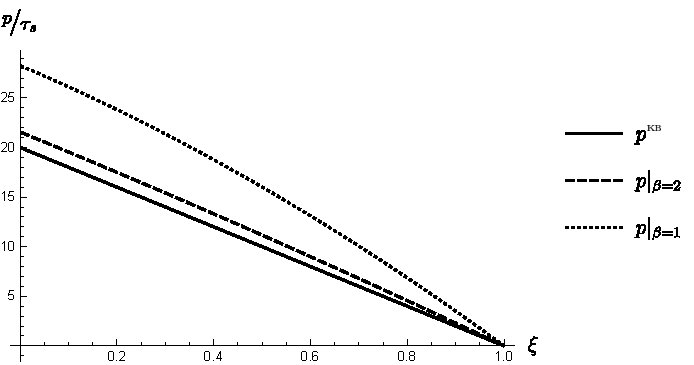
\includegraphics[width=0.9\linewidth]{./ch2/pressure_sub1}
  }
  \caption{Эпюры давления для случая цилиндрического слоя при радиусах цилиндров порядка толщины слоя}
  \label{fig:ch2/sub1/pressure}
\end{figure}
\begin{figure}[ht]
  \centerfloat{
    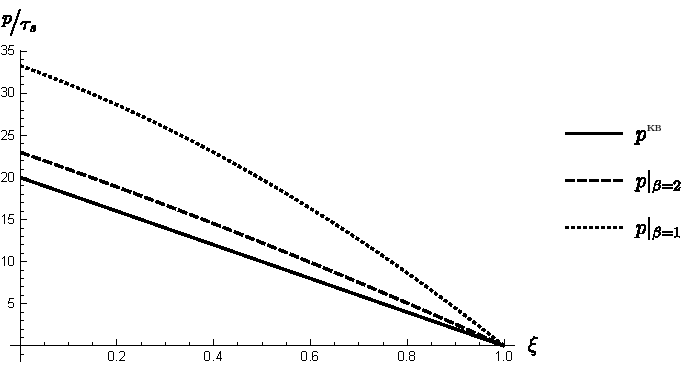
\includegraphics[width=0.9\linewidth]{./ch2/pressure_sub2}
  }
  \caption{Эпюры давления для случая цилиндрического слоя при радиусах цилиндров порядка длины образующей}
  \label{fig:ch2/sub2/pressure}
\end{figure}

Последний из рассматриваемых случаев, в силу наличия в уравнениях членов с дробными степенями параметра $\alpha$, требует использования иных разложений:
\begin{gather}
  v_{r}\left(r, z, t\right) = V \left(\uindex{v}{0}_{r} + \alpha^{1-c} \;\ \uindex{v}{1-c}_{r} + \cdots\right),
  \\
  v_{z}\left(r, z, t\right) = V \left(\alpha^{-1} \;\, \uindex{v}{-1}_{z} + \alpha^{-c} \;\, \uindex{v}{-c}_{z} + \uindex{v}{0}_{z} + \alpha^{1-c} \;\ \uindex{v}{1-c}_{z} + \cdots\right),
  \\
  s_{ij}\left(r, z, t\right) = \tau_{s} \left(\uindex{s}{0}_{ij} + \alpha^{1-c} \;\ \uindex{s}{1-c}_{ij} + \cdots\right),
  \\
  p\left(r, z, t \right) = \tau_{s} \left(\alpha^{-1} \;\, \uindex{p}{-1} + \alpha^{-c} \;\, \uindex{p}{-c} + \uindex{p}{0} + \alpha^{1-c} \;\ \uindex{p}{1-c} + \cdots\right).
\end{gather}
Поскольку однозначно определить порядок следующего за $\alpha^{1-c}$ члена не представляется возможным, поиск решения ограничен определением коэффициентов при $\alpha^{-1}$, $\alpha^{-c}$, $\alpha^0$ и $\alpha^{1-c}$. В силу данного ограничения падает точность искомых решений, и функция давления претерпевает изменения только в процессе развитого динамического деформирования:

\begin{gather}
  \begin{multlined}
    p^\text{кв} / \tau_{s} = p_0 + \frac{2\mu}{\alpha}\left(1-\lvert\xi\rvert\right) -\sqrt{1-\mu^2\left(2\rho-1\right)^2} \unl{+}
    \alpha^{1-c}\left( \vphantom{\frac{1-\mu^2\left(2\rho-1\right)\left(4\rho-1\right)}{\sqrt{1-\mu^2\left(2\rho-1\right)^2}}}
    \frac{1}{4\mu}\left(\mu\left(2\rho-1\right)\sqrt{1-\mu^2\left(2\rho-1\right)^2}+\arcsin{\left(\mu\left(2\rho-1\right)\right)}\right) \unl[1]{-}
    \frac{1-\rho}{2a}\frac{1-\mu^2\left(2\rho-1\right)\left(4\rho-1\right)}{\sqrt{1-\mu^2\left(2\rho-1\right)^2}}
    \right) +
    O(\alpha^{1-c}),
  \end{multlined}
  \\
  p\lvert_{\beta=1} = p^\text{кв} + \frac{3C_1}{2\alpha} \left(1-\xi^2\right) \tau_{s} + \frac{C_1}{2a \alpha^{c}}\left(3+2c\right)\xi^2 \tau_{s}.
\end{gather}
На \cref{fig:ch2/sub3/pressure} представлены эпюры давления для различных стадий процесса при $\alpha=0.1$, $C_1=1$, $c=0.5$, $\mu=1$ и $a=1$.
\begin{figure}[ht]
  \centerfloat{
    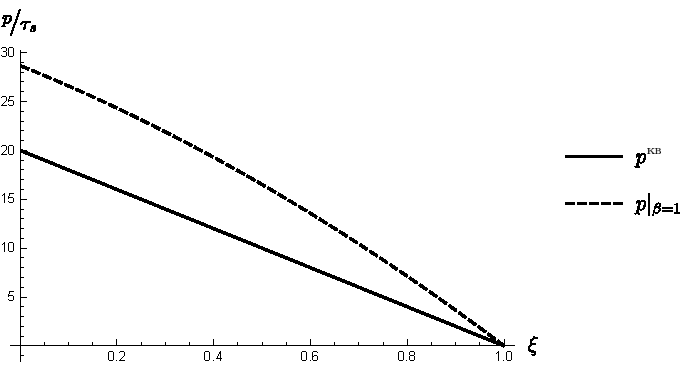
\includegraphics[width=0.9\linewidth]{./ch2/pressure_sub3}
  }
  \caption{Эпюры давления для случая цилиндрического слоя при радиусах ``промежуточного'' порядка}
  \label{fig:ch2/sub3/pressure}
\end{figure}

Во всех рассмотренных случаях прослеживается качественное изменение функции давления: возникает квадратично зависящее от продольной координаты слагаемое, причем порядок данной величины растёт с приближением к моменту ``схлопывания'' слоя.

\underline{\textbf{Третья глава}} посвящена исследованию влияния динамических эффектов в процессе сдавливания сферического идеально жесткопластического слоя \autocite{Shabaykin:2020a}.

Рассматривается течение несжимаемого слоя плотности $\varrho$, заключенного между двумя концентрическими сферами, в области
\begin{equation}
  \Omega_{t} = \{0 \le r \le R(t)+ h(t), 0 \le \theta < \pi, 0 \le \phi < 2\pi\}
\end{equation}
с границей $\partial\Omega = \Gamma = \Gamma_{1} \cup \Gamma_{2}$, причем $h(t) \ll R(t)$ для любого $t \ge 0$.

В процессе прессования внешняя сфера остаётся неподвижной, а внутренняя радиально расширяется с постоянной скоростью, выдавливая материал через сток $\theta=\pi$ (\cref{fig:ch3/layer}).
\begin{figure}[ht]
  \centerfloat{
    \includegraphics[height=0.2\textheight]{./ch3/layer}
  }
  \caption{Деформируемый сферический слой}
  \label{fig:ch3/layer}
\end{figure}

Система уравнений идеальной пластичности для данной задачи имеет вид:
\begin{gather}
  \begin{multlined}
    -p_{,r}+s_{rr,r}+\frac{1}{r}\left(s_{r\theta,\theta}+3s_{rr}+s_{r\theta}\cot{\left(\theta\right)}\right) \unl{=}
    \varrho \left(v_{r;t}+v_{r} v_{r,r} + \frac{1}{r}v_{\theta} v_{r,\theta} - \frac{1}{r} v_{\theta}^2 \right)
  \end{multlined},
  \\
  \begin{multlined}
    -\frac{1}{r} p_{,\theta}+s_{r\theta,r}+\frac{1}{r}\left(s_{\theta\theta,\theta}+3s_{r\theta}+\left(s_{rr}+2s_{\theta\theta}\right)\cot{\left(\theta\right)}\right) \unl{=}
    \varrho \left(v_{\theta;t}+v_{r} v_{\theta,r} + \frac{1}{r}v_{\theta} v_{\theta,\theta} - \frac{1}{r} v_{\theta} v_{r} \right)
  \end{multlined},
  \\
  s^2_{rr}+s^2_{\theta\theta}+s_{rr} s_{\theta\theta} + s^2_{r\theta}=\tau^2_{s}, \quad s_{rr} \left(v_{\theta,\theta} + v_{r}\right) / r = s_{\theta\theta} v_{r,r},
  \\
  s_{rr} \left(v_{\theta,r}+\left(v_{r,\theta}-v_{\theta}\right) / r\right) = 2 s_{r\theta} v_{r,r}, \quad v_{r,r}{+}\left(2v_{r}{+}v_{\theta,\theta}{+}v_{\theta}\cot{\left(\theta\right)}\right) / r = 0.
\end{gather}

На границах контакта $\Gamma_1$ и $\Gamma_2$ задаются кинематические и силовые граничные условия:
\begin{equation}
  v_{r}\lvert_{r=R} = V, \quad v_{r}\lvert_{r=R + h} = 0, \quad \lvert s_{r\theta}\lvert_{r=R} = \lvert s_{r\theta}\lvert_{r=R+h} = \mu(\theta) \tau_{s}, \quad 0 < \mu \le 1,
\end{equation}
где $\mu$ -- шероховатость пресса. Абсолютной шероховатости, или полному сцеплению пресса с материалом, соответствует значение $\mu = 1$.

Отыскание решения проводится методом асимптотического интегрирования. Вводятся малый параметр $\alpha = \frac{h(t)}{R(t)} \ll 1$ и безразмерные координаты
\begin{equation}
  \rho = \frac{r-R}{h}, \quad \tau = V \frac{t}{h}.
\end{equation}

Неизвестные функции представляются в виде степенных рядов, коэффициенты которых безразмерны и являются функциями безразмерных координат:
\begin{gather}
  v_{\theta}\left(r, \theta, t\right) = V \sum_{k=-1}^{\infty}{\alpha^{k} \; \uindex{v}{k}_{\theta}}, \quad v_{r}\left(r, \theta, t\right) = V \sum_{k=0}^{\infty}{\alpha^{k} \; \uindex{v}{k}_{r}},
  \\
  s_{ij}\left(r, \theta, t\right) = \tau_{s} \sum_{k=0}^{\infty}{\alpha^{k} \; \uindex{s}{k}_{ij}}, \quad p\left(r, \theta, t \right) = \tau_{s} \sum_{k=-1}^{\infty}{\alpha^{k} \; \uindex{p}{k}}.
\end{gather}

При подстановке данных разложений в уравнения движения возникает множитель $\text{Eu}^{-1}=\varrho V^2/\tau_s$ равный обратному числу Эйлера. Степень влияния учета динамики на протекание процесса определяется соотношением $\text{Eu}^{-1} \sim O(\alpha^\beta)$.
В рамках исследуемых стадий ($\beta=2$ и $\beta=1$) качественно меняется только функция давления. В случае квазистатической постановки она выражается в следующем виде:
\begin{equation}
  p^\text{кв} = p_0 - \tau_{s} \frac{2}{\alpha}\int_0^\theta \mu(\xi) d\xi + s_{rr} + O(1),
\end{equation}
где $p_0$ имеет смысл гидростатического давления.

Для стадии перехода от квазистатического режима к динамическому и стадии развитой динамики имеем соответственно выражения:
\begin{gather}
  p\lvert_{\beta=2} = p^\text{кв} + \tau_{s} C_2 \left(2\log{\left(\cos{\left({\theta / 2}\right)}\right)} - \frac{1}{1+\cos{\left(\theta\right)}}\right),
  \\
  p\lvert_{\beta=1} = p^\text{кв} + \frac{\tau_{s}}{\alpha} C_1 \left(2\log{\left(\cos{\left({\theta / 2}\right)}\right)} - \frac{1}{1+\cos{\left(\theta\right)}}\right) + O(1).
\end{gather}

При сравнении выражений видно, что в случае динамического сдавливания возникает дополнительное слагаемое, причем с уменьшением показателя $\beta$ его вклад возрастает. Функция
\begin{equation*}
  2\log{\left(\cos{\left({\theta / 2}\right)}\right)} - 1/\left(1+\cos{\left(\theta\right)}\right)
\end{equation*}
является выпуклой вверх при $\theta \in [0, \pi]$, причем её максимум достигается при $\theta=0$.
Наличие такого слагаемого качественно меняет эпюру давления в слое и увеличивает суммарную силу, действующую со стороны слоя на плиты.
Графики функции давления при $\alpha=0.1$, $C_1=1$, $C_2=2$, $\mu=1$ приведены на \cref{fig:ch3/sec3/pressure}.
\begin{figure}[ht]
  \centerfloat{
    \includegraphics[width=0.9\linewidth]{./ch3/pressure}
  }
  \caption{Эпюры давления для случая сферического слоя}
  \label{fig:ch3/sec3/pressure}
\end{figure}

В \underline{\textbf{четвертой главе}} исследуется влияние динамических эффектов в процессе сдавливания плоского нелинейно вязкопластического слоя со степенной функцией упрочнения \autocite{Shabaykin:2021b}.

Рассматривается течение несжимаемого вязкопластического материала, происходящее в тонком прямоугольном слое
\begin{equation}
  \Omega_{t} = \{-l(t) \le x_{1} \le l(t), -h(t) \le x_{2} < h(t)\}
\end{equation}
с границей $\partial\Omega = \Gamma = \Gamma_{1} \cup \Gamma_{2} \cup \Gamma_{3} \cup \Gamma_{4}$, причем $h(t) \ll l(t)$ для любого $t \ge 0$.
В начальный момент времени область, занятая материалом, имела вид
\begin{equation}
  \Omega_{0} = \{-l_{0} \le x_{1} \le l_{0}, -h_{0} \le x_{2} \le h_{0}\}, \quad \partial\Omega_{0} = \Gamma_{0}.
\end{equation}
Длинные стороны слоя соприкасаются с движущимися навстречу друг другу с постоянной скоростью $V$ плитами с коэффициентом шероховатости $\mu$ (\cref{fig:ch4/layer}).
\begin{figure}[ht]
  \centerfloat{
    \includegraphics[height=0.2\textheight]{./ch4/layer}
  }
  \caption{Деформируемый слой}
  \label{fig:ch4/layer}
\end{figure}

Замкнутая система плоской динамической теории вязкопластического течения состоит из пяти уравнений:
\begin{gather}
  -p_{,1}+s_{11,1}+s_{12,2} = \varrho \left(v_{1;t}+v_{1} v_{1,1} + v_{2} v_{1,2} \right),
  \\
  -p_{,2}-s_{11,2}+s_{12,1} = \varrho \left(v_{2;t}+v_{1} v_{2,1} + v_{2} v_{2,2} \right),
  \\
  \sqrt{s^2_{11}+s^2_{12}}=\sigma_{s} + 2 a v_{u}^\gamma, \quad v_{u} = \sqrt{2 v^2_{1,1}+\left(v_{1,2}+v_{2,1}\right)^2 / 2},
  \\
  s_{11} \left(v_{1,2}+v_{2,1}\right) = 2 s_{12} v_{1,1},\quad v_{1,1}+v_{2,2} = 0,
\end{gather}
где $\varrho$ -- плотность материала, $a$ -- коэффициент нелинейной вязкости и $\gamma$ -- экспонента упрочнения.

На границах контакта $\Gamma_1$ и $\Gamma_2$ задаются кинематические и силовые граничные условия:
\begin{equation}
  \label{eq:ch4/sec1/boundary/kinematic}
  v_{2}\lvert_{x_2\pm h} = \mp V, \quad \lvert s_{12}\lvert_{x_2=\pm h} = \mu(x_1) \tau_{s}, \quad 0 < \mu \le 1.
\end{equation}

Вводится малый геометрический параметр $\alpha=\frac{h(t)}{l(t)}\ll 1$, и неизвестные функции раскладываются в ряды по целым степеням параметра:
\begin{gather}
  v_{1}\left(x_1, x_2, t\right) = V \sum_{k=-1}^{\infty}{\alpha^{k} \; \uindex{v}{k}_{1}}, \quad v_{2}\left(x_1, x_2, t\right) = V \sum_{k=0}^{\infty}{\alpha^{k} \; \uindex{v}{k}_{2}}
  \\
  s_{ij}\left(x_1, x_2, t\right) = \tau_{s} \sum_{k=0}^{\infty}{\alpha^{k} \; \uindex{s}{k}_{ij}}, \quad p\left(x_1, x_2, t\right) = \tau_{s} \sum_{k=-1}^{\infty}{\alpha^{k} \; \uindex{p}{k}},
\end{gather}
где коэффициенты рядов безразмерны и являются функциями безразмерных координат $\xi_1, \xi_2, \tau$:
\begin{equation}
  \xi_1 = x_1 / l = \alpha x_1 / h, \quad \xi_2 = x_2 / h, \quad \tau = V \frac{t}{h}.
\end{equation}

Подстановка данных разложений в уравнения движения порождает два параметра: малый физический параметр $\text{Eu}^{-1}=\varrho V^2/\tau_s$ равный обратному числу Эйлера -- ключевому безразмерному критерию в динамических задачах механики сплошных сред, и другой критерий подобия, число Сен-Венана  $\text{S}~=~\left(\tau_s/a\right) \left(h/V\right)^\gamma \gg 1$, описывающий отношение пластических и вязких свойств тела.
Посредством асимптотического интегрирования, с учетом соотношения $\text{Eu}^{-1} \sim O(\alpha^\beta)$, строится решения для двух стадий процесса: этапа перехода от квазистатического к динамическому деформированию ($\beta=2$) и этапу развитого динамического деформирования ($\beta=1$).

Полученные приближенные решения качественно отличаются от квазистатического случая только функцией давления:
\begin{gather}
  p^\text{кв}  = p_0 +  \frac{\tau_{s}}{\alpha}\int_{\vert \xi_1\vert}^1 \mu(\xi) d\xi - s_{11} + \int_{-1}^{1}{s_{11} d\xi_2} + O(\alpha),
  \\
  p\lvert_{\beta=2} = p^\text{кв} + \tau_{s} C_2 \left(1-\xi_1^2\right),
  \\
  p\lvert_{\beta=1} = p^\text{кв} + \frac{\tau_{s}}{\alpha} C_1 \left(1-\xi_1^2\right) + O(1),
\end{gather}
где $p_0$ имеет смысл гидростатического давления.

При сравнении выражений видно (\cref{fig:ch4/sec4/pressure}), что в случае динамического сдавливания возникает квадратично зависящее от радиуса слагаемое, причем чем меньше показатель $\beta$, тем более значима становится данная величина. Наличие такой зависимости качественно меняет эпюру давления в слое и увеличивает суммарную силу, действующую со стороны слоя на плиты.
\begin{figure}[ht]
  \centerfloat{
    \includegraphics[width=0.9\linewidth]{./ch4/pressure}
  }
  \caption{Эпюры давления для случая плоского вязкопластического слоя при параметрах $\alpha=0.1$, $C_1=1$, $C_2=2$, $\mu=0.9$, $\text{S}=10$}
  \label{fig:ch4/sec4/pressure}
\end{figure}

\FloatBarrier
\pdfbookmark{Заключение}{conclusion}                                  % Закладка pdf
В \underline{\textbf{заключении}} приведены основные результаты работы, которые заключаются в следующем:
%% Согласно ГОСТ Р 7.0.11-2011:
%% 5.3.3 В заключении диссертации излагают итоги выполненного исследования, рекомендации, перспективы дальнейшей разработки темы.
%% 9.2.3 В заключении автореферата диссертации излагают итоги данного исследования, рекомендации и перспективы дальнейшей разработки темы.
\begin{enumerate}
  \item Получены приближенные аналитические решения в задаче о сдавливании круглого идеально жесткопластического тонкого слоя в динамической постановке. Рассмотрены две стадии процесса, соответствующие переходу от квазистатического к динамическому режиму деформирования и развитому динамическому деформированию.
  \item Получены приближенные аналитические решения в задаче о сдавливании цилиндрического идеально жесткопластического тонкого слоя в динамической постановке. В данной задаче естественно возникает дополнительный параметр, отвечающий за соотношение радиусов и длины образующей сжимающих цилиндров. Рассмотрены случаи, когда радиусы цилиндров имеют тот же порядок, что и толщина слоя, когда радиусы цилиндров порядка длины образующей, и случай ``промежуточного'' порядка. Для указанных случаев исследованы две стадии процесса прессования: переход от квазистатического к динамическому режиму деформирования и развитое динамическое деформирование.
  \item Получены приближенные аналитические решения в задаче о сдавливании сферического идеально жесткопластического тонкого слоя при наличии стока в динамической постановке. Показано что процесс прессования разбивается по времени на качественно различные стадии: этап соответствующий переходу от квазистатического к динамическому режиму деформирования и этап развитого динамического деформирования.
  \item Получены приближенные аналитические решения в задаче о сдавливании вязкопластического тонкого слоя со степенной функцией упрочнения в динамической постановке для режимов прессования, соответствующих стадии перехода от квазистатического к динамическому режиму деформирования и стадии развитого динамического деформирования.
  \item Анализ напряженно-деформированного состояния на исследуемых стадиях показал качественное изменение эпюры давление и увеличение суммарной силы действующей со стороны материала на прессующие поверхности: в функции давления возникло зависящее от продольной координаты слагаемое (выпуклая вверх функция с центром в северном полюсе в случае сферического слоя и квадратичная функция в остальных задачах), причем с приближением к моменту ``схлопывания'' слоя вклад данного слагаемого растет.
  \item Определена область применимости найденных решений и построен явный критерий, устанавливающий зависимость между временем и стадией процесса прессования. Согласно последнему независимо от малости постоянной скорости сближения жестких прессующих поверхностей наступает временной интервал, когда влияние динамических слагаемых становится соизмеримым с градиентами напряжений.
  \item Развит метод асимптотического интегрирования для динамических задач пластического течения при прессовании асимптотически тонких слоев.
\end{enumerate}


\pdfbookmark{Литература}{bibliography}                                % Закладка pdf

\ifdefmacro{\microtypesetup}{\microtypesetup{protrusion=false}}{} % не рекомендуется применять пакет микротипографики к автоматически генерируемому списку литературы
\urlstyle{rm}                               % ссылки URL обычным шрифтом
\ifnumequal{\value{bibliosel}}{0}{% Встроенная реализация с загрузкой файла через движок bibtex8
  \renewcommand{\bibname}{\large \bibtitleauthor}
  \nocite{*}
  \insertbiblioauthor           % Подключаем Bib-базы
  %\insertbiblioexternal   % !!! bibtex не умеет работать с несколькими библиографиями !!!
}{% Реализация пакетом biblatex через движок biber
  % Цитирования.
  %  * Порядок перечисления определяет порядок в библиографии (только внутри подраздела, если `\insertbiblioauthorgrouped`).
  %  * Если не соблюдать порядок "как для \printbibliography", нумерация в `\insertbiblioauthor` будет кривой.
  %  * Если цитировать каждый источник отдельной командой --- найти некоторые ошибки будет проще.
  %
  %% authorvak
  \nocite{vakbib1}%
  \nocite{vakbib2}%
  %
  %% authorwos
  \nocite{wosbib1}%
  %
  %% authorscopus
  \nocite{scbib1}%
  %
  %% authorpathent
  \nocite{patbib1}%
  %
  %% authorprogram
  \nocite{progbib1}%
  %
  %% authorconf
  \nocite{confbib1}%
  \nocite{confbib2}%
  %
  %% authorother
  \nocite{bib1}%
  \nocite{bib2}%

  \ifnumgreater{\value{usefootcite}}{0}{
    \begin{refcontext}[labelprefix={}]
      \ifnum \value{bibgrouped}>0
        \insertbiblioauthorgrouped    % Вывод всех работ автора, сгруппированных по источникам
      \else
        \insertbiblioauthor      % Вывод всех работ автора
      \fi
    \end{refcontext}
  }{
    \ifnum \totvalue{citeexternal}>0
      \begin{refcontext}[labelprefix=A]
        \ifnum \value{bibgrouped}>0
          \insertbiblioauthorgrouped    % Вывод всех работ автора, сгруппированных по источникам
        \else
          \insertbiblioauthor      % Вывод всех работ автора
        \fi
      \end{refcontext}
    \else
      \ifnum \value{bibgrouped}>0
        \insertbiblioauthorgrouped    % Вывод всех работ автора, сгруппированных по источникам
      \else
        \insertbiblioauthor      % Вывод всех работ автора
      \fi
    \fi
    %  \insertbiblioauthorimportant  % Вывод наиболее значимых работ автора (определяется в файле characteristic во второй section)
    \begin{refcontext}[labelprefix={}]
      \insertbiblioexternal            % Вывод списка литературы, на которую ссылались в тексте автореферата
    \end{refcontext}
    % Невидимый библиографический список для подсчёта количества внешних публикаций
    % Используется, чтобы убрать приставку "А" у работ автора, если в автореферате нет
    % цитирований внешних источников.
    \printbibliography[heading=nobibheading, section=0, env=countexternal, keyword=biblioexternal, resetnumbers=true]%
  }
}
\ifdefmacro{\microtypesetup}{\microtypesetup{protrusion=true}}{}
\urlstyle{tt}                               % возвращаем установки шрифта ссылок URL
